% This LaTeX was auto-generated from an M-file by MATLAB.
% To make changes, update the M-file and republish this document.

\documentclass[12pt]{article}
\usepackage{natbib}
\usepackage[french]{babel}
\usepackage[utf8x]{inputenc}
\usepackage[smartEllipses]{markdown}
\usepackage{lipsum}
\usepackage{amsmath}
\usepackage{hyperref}
\usepackage{tabularx}
\usepackage{multirow}
\usepackage{graphicx}
\usepackage[final]{pdfpages}
\usepackage[T1]{fontenc}
%\usepackage[colorinlistoftodos]{todonotes}
\usepackage{xcolor}
\usepackage[nottoc,numbib]{tocbibind}% Para que la bibliografia salga en el table of contents
\colorlet{Mycolor1}{green!10!orange!90!}
\usepackage{subfigure}
\usepackage{plantuml}
\sloppy
\definecolor{lightgray}{gray}{0.5}
\setlength{\parindent}{0pt}
\setlength{\parskip}{1em}

\bibliographystyle{abbrv}

\begin{document}
\title{Rapport stage ASTC}
\author{CHIRINO CAICEDO Melet}
\begin{titlepage}

\newcommand{\HRule}{\rule{\linewidth}{0.5mm}} % Defines a new command for the horizontal lines, change thickness here

\center % Center everything on the page
 
%----------------------------------------------------------------------------------------
%	HEADING SECTIONS
%----------------------------------------------------------------------------------------

\textsc{\LARGE Université Toulouse III}\\[0.5cm] % Name of your university/college
\textsc{\Large Paul Sabatier}\\[1.0cm] % Major heading such as course name
\textsc{\large Rapport du stage 2021/2022}\\[0.5cm] % Minor heading such as course title

%----------------------------------------------------------------------------------------
%	TITLE SECTION
%----------------------------------------------------------------------------------------

\HRule \\[0.4cm]
{ \huge \bfseries Integration d'un logiciel embarqu\'e AUTOSAR en simulation}\\[0.4cm] % Title of your document
\HRule \\[1.5cm]
 
%----------------------------------------------------------------------------------------
%	AUTHOR SECTION
%----------------------------------------------------------------------------------------

\begin{minipage}{0.4\textwidth}
\begin{flushleft} \large
\markboth{Pojet en \LaTeX}
\emph{Auteurs:}\\
\textsc{CHIRINO} Melet \\ % Your name
%\textsc{RIBEIRO} Bruno % Your name
\end{flushleft}
\end{minipage}
~
\begin{minipage}{0.5\textwidth}
\begin{flushright} \large
\emph{Tuteur:} \\
\textsc{BROUEILH} Nicolas  % Supervisor's Name
\textsc{RIVI\`ERE} Nicolas  % Supervisor's Name
\end{flushright}
\end{minipage}\\[2cm]

% If you don't want a supervisor, uncomment the two lines below and remove the section above
%\Large \emph{Author:}\\
%John \textsc{Smith}\\[3cm] % Your name

%----------------------------------------------------------------------------------------
%	DATE SECTION
%----------------------------------------------------------------------------------------

{\large \today}\\[1cm] % Date, change the \today to a set date if you want to be precise

%----------------------------------------------------------------------------------------
%	LOGO SECTION
%----------------------------------------------------------------------------------------


\includegraphics[width=6in]{img/Logo_UT3.jpg}\\[2cm] % Include a department/university logo - this will require the graphicx package
 
%----------------------------------------------------------------------------------------

\vfill % Fill the rest of the page with whitespace

\end{titlepage}

%\{Contents}
\tableofcontents

\newpage

%-------------------------- * Introduccion * --------------------------------

\section{Introduction}
\section{Introduction}

\subsection{Description de la societ\'e}
Australian Semiconductor Technology Company (ASTC) est un fournisseur mondial des solutions logicielles et matériels pour les systèmes embarqués. Cette soci\'et\'e propose des services de conception, validation et vérification des systèmes sur puces et les circuits intégrés. Elle a développé son outil VLAB, qui fournit des solutions innovantes, pour la simulation des logiciels embarqués sur les plateformes Hardware virtuelles. La société a son siège à Adélaïde en Australie, elle possède des bureaux et des centres de R\&D à Toulouse, Tokyo, Illinois, Austin, et Texas. 

ASTC Desing partners a été créée \`a toulouse par Nicolas Broueilh et Eric Faure en 2014. Cette partie est plus focalis\'e en la conception de logiciel embarqu\'e, sourtout la virtualisation de hardware avec VLAB Works. Le produit le plus develop\'e est la toolbox \textit{AURIX} qui est capable de virtualiser la famille \textit{aurix} de \textit{Infineon Technologies AG}. Dans la figure \ref{fig:vlab-presentation} on peut voir un exemple de vlab.

VLAB utilise python2 pour accéder a tous les éléments de hardware virtuel et évènements de la simulation comme les ports du microcontroleur, registres, connections entre mod\`eles, temps de simulation, points d'arrête, etc. Pour les modèles de simulation il est utilis\'e C++ avec la librairie SystemC. Il y existe une API de SystemC pour python2 en raison de développer des mod\`eles plus rapidement mais moins performantes que celles en SystemC. Toutes les mod\`eles doivent \^etre compil\'es avant de d\'emarrer la simulation.

%Para programar en vlab es necesario usar python2 y con este podemos acceder a todos los elementos de la simulacion. Para los modelos es necesario hacerlo usando C++ y SystemC. Hay una API de SystemC para python lo cual permite hacer pequenhos modelos mas rapido pero eso tendra un impacto en la velocidad de la simulacion si no son compilados. Para los modelos que necesitan mas performance es mejor usar SystemC.

%Aqui empiezo hablando de que es astc, que es una empresa internacional que hace herramientas de simulacion de microcontroladores. Explico un poco que es vlab, un par de capturas de pantalla con la que se muestre sus caracteristicas funcionales y zas, juera. 

%Finalmente digo que mi stage se trata de modelizar un gateway ya existente con la herramienta de simulacion.

\begin{figure}[!htb]
    \centering
        \subfigure[Vlab Logo]{
\includegraphics [width=2.5in]{img/VLAB_Works.png}}
        \subfigure[Vlab en marche]{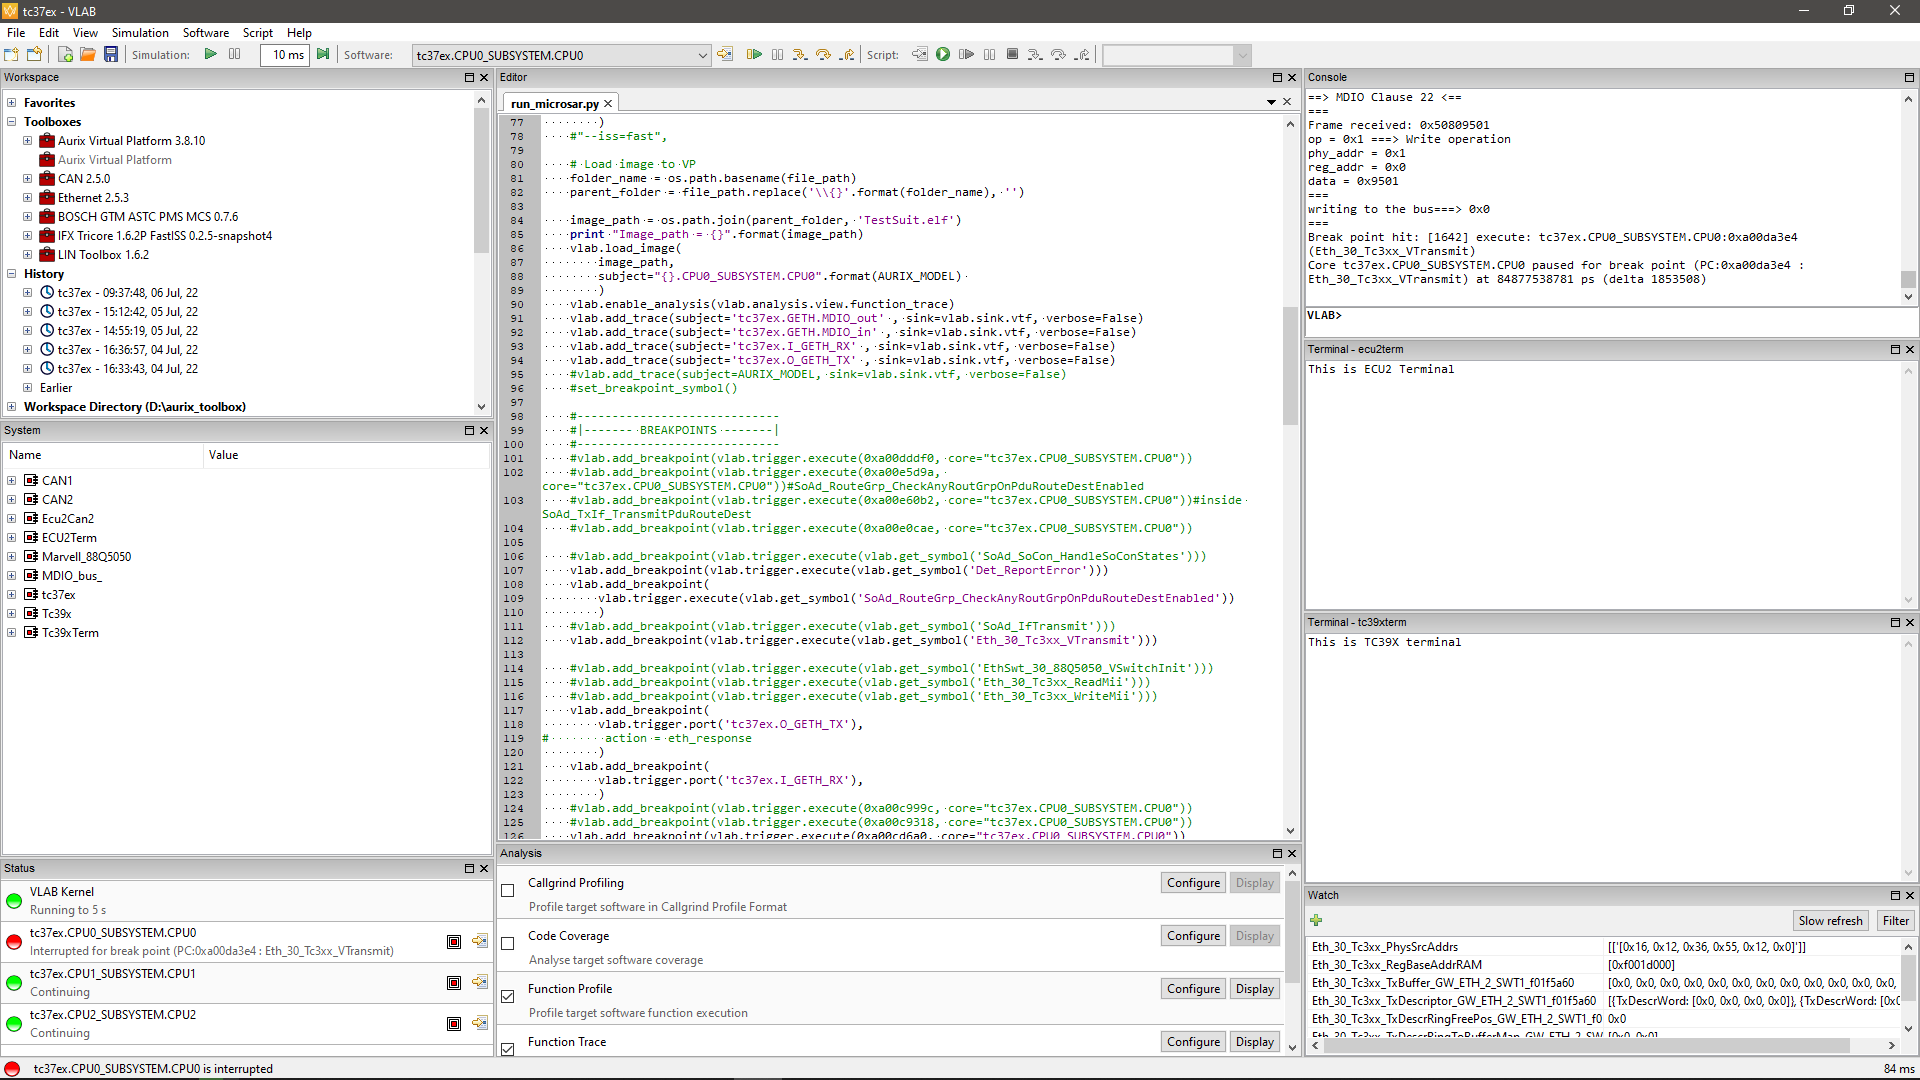
\includegraphics [width=5in]{img/vlab.png}}
    \caption{Vlab works}
    \label{fig:vlab-presentation}
\end{figure}

%\subsection{Virtualizacion y sus ventajas}


%-------------------------- * Descripcion * --------------------------------

\section{Cadre du projet et probl\'ematique}
\section{Cadre du projet et probl\'ematique}

\subsection{Description du projet}

Une Gateway est un noeud dans un réseau qui se communique avec un réseau extérieur \cite{gateway-definition}. Cette gateway permet de communiquer différents types de réseaux dans une voiture pour connecter plusieurs ECU's qui n'appartient pas au même reseau comme la CAN, LIN, Ethernet ou m\^eme 5G. 

La societe \textit{Infineon Technologie GA} a developp\'e un gateway securis\'e automobile avec la reference KIT\_A2G\_TC377\_SEC\_GTW \cite{gateway} (fig \ref{fig:gw-photo}) qui utilise un microcontr\^oleur \textit{AURIX TC37xEXT} pour connecter les differents reseaux internes d'une voiture comme FlexRay, LIN, CAN ou Ethernet. Le syst\`eme d'exploitation pour cette gateway s'appelle MICROSAR Classic \cite{vector.microsar} et est fourni par Vector Informatik. Ce Syst\`eme d'explotation est compatible avec les standards AUTOSAR\cite{autosar-intro} donc le develeoppeur peut utiliser des <<software components>>\footnote{Dans la notation AUTOSAR les fonctions de la couche la plus haute d'abstraction sont appel\'es software components ou SWC\cite{swc_man}.} Autosar dans ce version de MICROSAR.

Inclus dans la gateway, il se trouve un switch Ethernet securis\'e Marvell 88Q5050 qui a des connections Gigabit Ethernet en différents standards de l'industrie. Cette gateway nous offre une solution de connections en differents reseaux de la voiture totalement compatible avec AUTOSAR a differents vitesses de fonctionement et avec une haute degré de securit\'e. Dans le cas qu'une ECU connect\'e a la reseaux CAN demande certain information d'un Camera qui envoie des donn\'ees par Gigabit Ethernet ce communication sera possible en contr\^ol\'e par le developpeur en fonction de priorit\'es du syst\`eme.

%La societe \textit{Infineon Technologie GA} a developp\'e un gateway securis\'e automobile avec la reference KIT\_A2G\_TC377\_SEC\_GTW \cite{gateway} (fig \ref{fig:gw-photo}) el cual corre con un microcontrolador \textit{AURIX TC37xEXT} para poder aumentar la conectividad de diferentes redes como el FlexRay, LIN, CAN y Ethernet dentro del automobil. El sistema operativo usado dentro de este gateway es fourni por Vector Informatik y se llama MICROSAR Classic \cite{vector.microsar}. Este sistema operativo es totalmente compatible con AUTOSAR lo cual nos deja con una ECU 100\% funcional sobre la cual se pueden correr software components (swc) compatibles con AUTOSAR. Ademas tambien se utilisa un switch ethernet securis\'e Marvell 88Q5050 que permite velocidad y ancho de banda estables con toda la seguridad que un automobil requiere.

\begin{figure}[!htb]
 \centering
 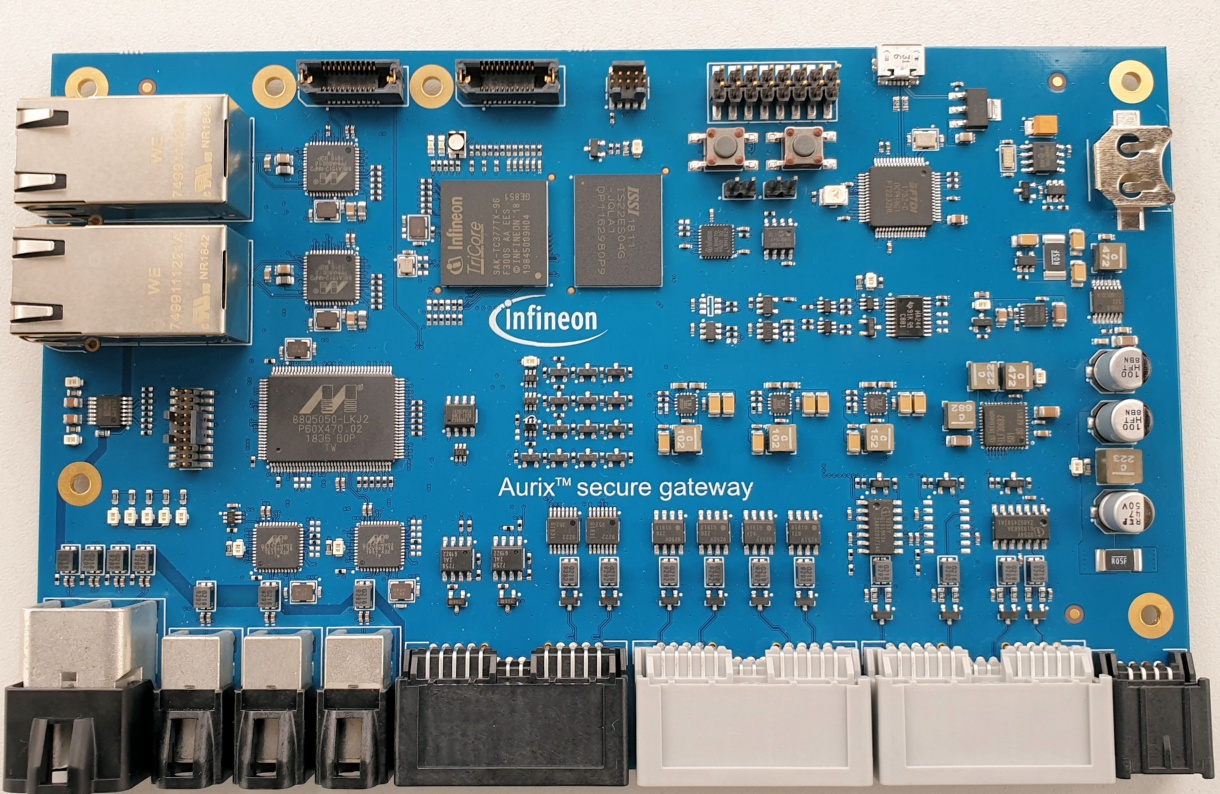
\includegraphics[width=0.8\textwidth]{img/secure-gateway.jpg}
 \caption{KIT\_A2G\_TC377\_SEC\_GTW}
 \label{fig:gw-photo}
\end{figure}

Le syst\`eme d'exploitation est fournie avec une petite demo technique qui sert pour la prise en main de la gateway et tester son fonctionnement basique de connecter 2 reseaux avec des protocoles physiques et logiques incompatibles. Pour lancer la demo il est necessaire de connecter 2 ECU externes \`a certains ports CAN et Ethernet du gateway, voir figures \ref{fig:gw-demo-uc1} et \ref{fig:gw-demo-uc2} pour plus d'information concernant aux connections. La demo a 2 cas d'utilisation :

%El gateway viene con un programa de demostracion que pretende hacer la prise en main del gateway, testear el funcionamiento basico y mostrar las capacidades del mismo. Para testear el Demo es necesario conectar 2 ECU's externar a ciertos puertos especificados en la figura \ref{fig:connections-diagram}. El demo en cuestion tiene 2 use Cases los cuales vamos a explicar por separado.

\begin{itemize}
    \item Use Case 1 : L'ECU connect\'e au port CAN envoie une trame d'information qui sera reenvoy\'e vers l'ECU en Ethernet (fig. \ref{fig:gw-demo-uc1}).%En este Use Case se envia un frame can y el gateway le hace forward por puerto ethernet. Retratado en la figura \ref{fig:gw-demo-uc1}.
    \item Use Case 2 : L'ECU connect\'e au port Ethernet envoie une trame d'information qui sera reenvoy\'e vers l'ECU en CAN (fig. \ref{fig:gw-demo-uc2}).%En Este Use case se envia un frame ethernet y esto se le hace forward hacia un bus can. Retratado en la figura \ref{fig:gw-demo-uc2}.
\end{itemize}

\begin{figure}[!htb]
 \centering
 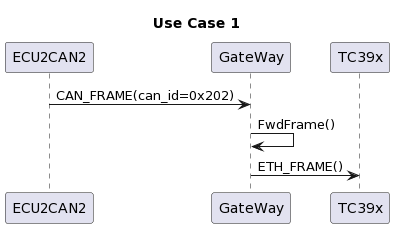
\includegraphics[width=0.5\textwidth]{img/GWUseCase1.png}
 \caption{Gateway Demo Use Case 1}
 \label{fig:gw-demo-uc1}
\end{figure}

\begin{figure}[!htb]
 \centering
 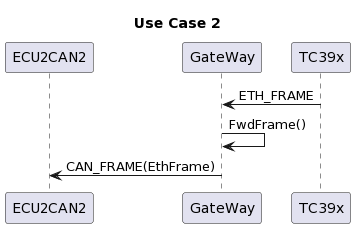
\includegraphics[width=0.5\textwidth]{img/GWUseCase2.png}
 \caption{Gateway Demo Use Case 2}
 \label{fig:gw-demo-uc2}
\end{figure}

Pour tester le fonctionnement basique de cette gateway il nous faut toute une infrastructure comme une reseaux CAN, des ECU compatibles, un banc de tests, outils de vérification, etc, ce nous présente les probl\`emes suivants:
\begin{itemize}
    \item - Construction d'une espace contr\^ol\'e et securis\'e pour accueillir ces composants.
    \item - Haute coûte d'achats des composants pour tester qui pourront ne pas être disponibles vu la situation actuelle des semiconducteurs.
    \item - Fabrication des bancs de test.
    \item - Frais des maintenance future pour maintenir le bon fonctionnement du banc de test.  
\end{itemize}

Toute ces probl\`emes augmentent le co\^ut et la dur\'ee du projet, et si les besoins du projet changent il sera nécessaire changer des composants ou fabriquer des nouvelles pièces de hardware. Dans une cadre du développement de logiciel ce n'est pas le cas le plus efficace.

\subsection{Objectifs du projet}

ASTC Design Partners veut virtualiser cette gateway en utilisant son outil VLAB Works. Avec une solution virtualis\'e non seulement les coûts de fabrication, délais de livraison et maintenance seront evit\'es mais aussi le développement de tests automatis\'es sera plus rapide, chaque développeur aura son propre banc de test personalis\'es et les bugs software seront trouves plus facilement. 

%La propuesta de ASTC Desing Partners es virtualizar este Gateway para poder agilizar el proceso del desarrollo de software, sobretodo en un contexto de escasez mundial de microcontroladores. Ademas, es bien sabido que suele haber pocas unidades disponibles para testear por lo que es mejor tenerlo digitalizado para que cada programador pueda avanzar por su lado sin necesidad de hacer cola por el hardware, a menos que sea necesario.

Au début du projet nous avions disponible VLAB, le mod\`ele virtualis\'e du microcontr\^oleur \textit{AURIX TC37x} utilis\'e dans la gateway et le software compil\'e MICROSAR fournie avec la gateway. Le software de la gateway doit verifier le fonctionement correct de toutes les componsants et buses de donn\'ees presents sur la gateway. A fin de virtualiser la gateway, il faut remplir quelques objectifs basiques : 
\begin{itemize}
    \item - Modéliser des composants nécessaires pour que le syst\`eme d'exploitation démarre.
    \item - Faire un testbench avec les bus de donn\'ees necessaires pour l'envoie des donn\'ees.
    \item - Augmenter les capacit\'es du \textit{TC37x} parce que la gateway utilise une version amelior\'e de ce microcontr\^oleur appell\'e par infineon \textit{TC37xEXT}\cite{aurix.tc37e}.
\end{itemize}
%
%-------------------------- * Objetivos * --------------------------------

\section{Objectifs}
Mis objetivos... Debo preguntarle a Nico por mis objetivos precisos pero yo diria 
\begin{itemize}
    \item cargar microsar sobre un tc37x simulado y hacer que arranque
    \item Imitar las funcionalidades de canoe
    \item Hacer una UI (en pygame papu, eso me va a quedar para toda la vida)
\end{itemize}

%-------------------------- * Estado del Arte * --------------------------------
\section{Etat de l'Art}
Aqui vas a explicar los conceptos fundamentales para entender todo lo que se va a explicar en el desarrollo como: AUTOSAR, VECTOR Microsar, Virtualizacion, nuestro gateway, redes ETH, CAN, LIN, Fr, vlab, 

%-------------------------- * Conception/Desarrollo * --------------------------------
\section{Conception}
\section{Conception}

Avant la conception du projet il est nécessaire la prise en main du logiciel VLAB et l'utilisation des toolbox disponibles comme le toolbox CAN, Ethernet, LIN et aurix. J'ai d'abord instal\'e l'environement du travail avec les identifiants pour acceder \`a la reseaux interne de la soci\'et\'e. Deuxièmement, j'ai telecharge les dossiers du travail depuis les servers d'Australie. Apr\`es, j'ai compil\'e du logiciel simple pour tester le microcontr\^oleur (désormais appel\'e \textit{aurix}). Finalement, j'ai mod\'elis\'e quelques composants génériques pour tester des autres fonctionalit\'es du VLAB comme les connections des bancs de test, l'envoie de donn\'ees a travers des différents réseaux et la réception et utilisation de donn\'ees. Le développement de ce projet a \'et\'e divis\'e en 3 parties en fonction de l'évolution du même.

\begin{itemize}
    \item - Premier demo technique qui sers a faire la prise en main d'AUTOSAR, VLAB et l'environnement en général.
    \item - Developpement de l'aurix \textit{TC37xEXT}\cite{aurix.tc37e}, pas support\'e jusqu'\`a moment du démarrage du stage.
    \item - Virtualisation du Gateway
\end{itemize}

\subsection{Premier demo technique}

Le premier exemple est fait pour tester le logiciel avec une configuration super simple. Il consiste a envoyer une trame CAN et le SWC la reenvoie vers le CANID source. Pour cet exemple une ECU générique a \'et\'e modélisé pour recevoir des trames CAN et LIN. Sur la figure \ref{fig:first-demo-diagram} se montre un diagrame de block des communications. Le code de ces ECUs se trouve dans l'anexe \ref{anexe:hybrid_node}.

\begin{figure}[!htb]
 \centering
 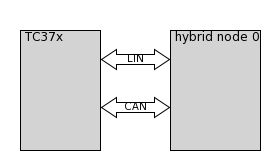
\includegraphics[]{img/first_demo_testbench.png}
 \caption{Premier demo}
 \label{fig:first-demo-diagram}
\end{figure}

Le structure de communications d'AUTOSAR de la figure \ref{fig:autosar-com-stack} nous montre que le chemin parcouru par les donn\'ees arrivant \'a l'aurix. Le chemin des donn\'ees de cette premier demo est le suivant \textit{Microcontroler}$ ->$ \textit{CAN\_Driver}\cite{can_drv_man} $->$ \textit{CAN\_IF}\footnote{IF dans la notation AUTOSAR veut dire Interface}\cite{can_if_man} $->$ \textit{PDU-R}\footnote{PDU est le nom des donn\'ees dans cette couche d'abstraction selon le mod\`ele OSI\cite{osi-model}.}\footnote{PUD-R\cite{pdu_r_man} est le router des PDUs. C'est ce module qui prends le décision o\`u envoyer les donn\'ees re\c cues}\cite{pdu_r_man}. C'est ici dans le PDU-R qu'on trouve un probl\`eme parce que la trame re\c cue n'est pas activ\'e au début du programme.

Cette première demo a \'et\'e con\c cue pour \^etre test\'e avec le logiciel \textbf{CANoe}\cite{canoe} dont nous ne possédions pas la licence et le SWC n'a pas march\'e comme attendu. Les possibles explications sont las suivantes :

\begin{itemize}
    \item - Un protocole inconnu : Même si CANoe utilise le protocole CAN, il envoie peut \^etre d'autres trames d'identification avant le test.
    \item - Un SWC peu test\'e : Selon la documentation de ce test, ce SWC n'a pas \'et\'e teste au fond parce que son utilisation ne sera jamais implement\'e, c'est juste un test des logiciels.
\end{itemize}

\begin{figure}[!htb]
 \centering
 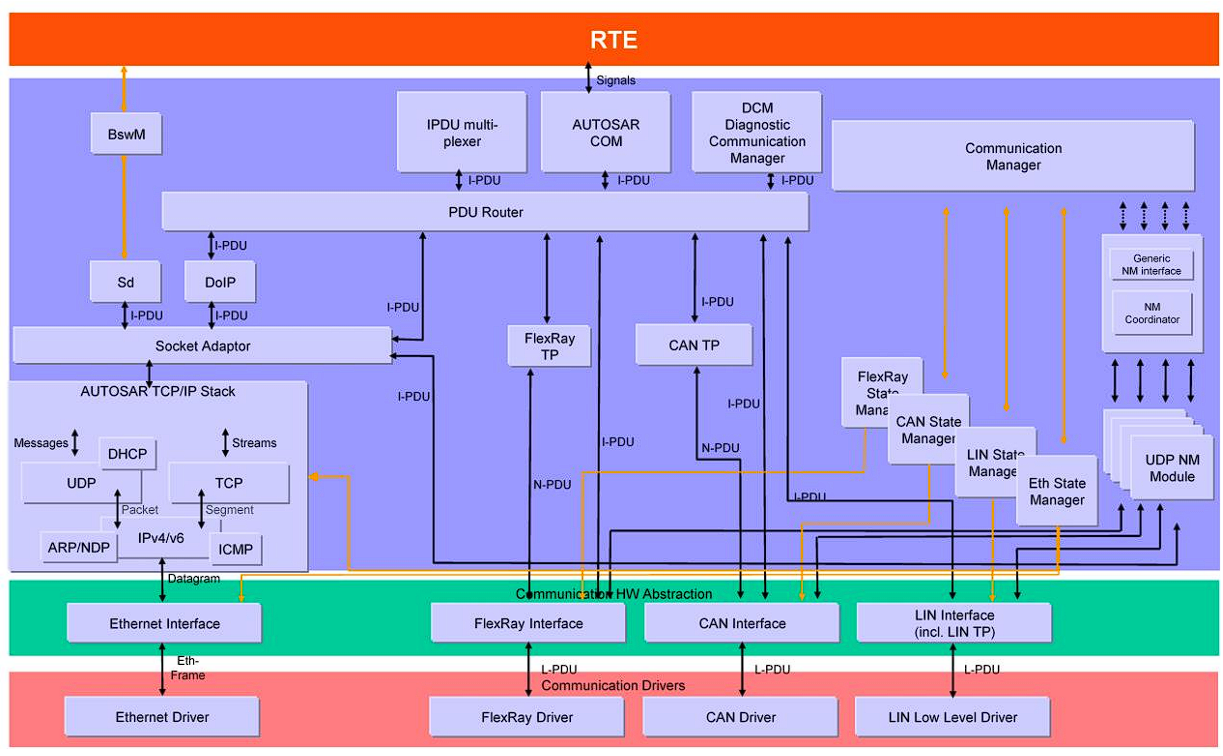
\includegraphics[width=\textwidth]{img/autosar_com_stack.png}
 \caption{Autosar Communication Stack\cite{sock_adp_man}}
 \label{fig:autosar-com-stack}
\end{figure}

Quand même, avec ce test j'ai acquis une connaissance basique du fonctionnement des logiciels AUTOSAR ce qui a rendu mon travaille future plus rapide et efficace. Un autre connaissance acquis dans ce partie c'était la partie de modélisation et le modèle de ECU déjà développe sera utilise plus tard.

\subsection{TC37xEXT}

Cette version de l'aurix ajoutait quelques modules de plus, les plus concernant pour ce projet c'etaient une interface CAN (MCMCAN\footnote{C'est le nom de l'interface CAN dans la famille de microcontroleurs \textit{aurix}}) et Gigabit Ethernet (GETH) de plus. Les autres differences seront trouv\'ees dans la table \ref{tab:tc37x_delta}. Le modèle du \textit{TC37x}\cite{aurix.tc37x} a \'et\'e pris comme la base et les interfaces et modules ont \'et\'e ajout\'es selon les adresses de base sur les buses correspondants.


% Table generated by Excel2LaTeX from sheet 'Sheet1'
\begin{table}[htbp]
  \centering
    \begin{tabular}{|r||l|l|}
	\hline
	\multirow{2}{*}{Module} & \multicolumn{2}{c|}{Aurix}\\
	\cline{2-3}
	& TC37x & TC37xEXT \\
	\hline \hline
	    RAM & TRAM (cached, non-cached) & EMEM (cached, non-cached) \\
	    \hline
	    CAN interfaces & 2 & 3 \\
	    \hline
	    Camera Interface & not present & CIF \\
	    \hline
	    Gigabit Ethernet Interface & 1 & 2 \\
	    \hline
	    SD interface & not present & present \\
	    \hline
	    eMMC interface & not present & present \\
	    \hline
	\hline
    \end{tabular}
  \caption{TC37x Vs TC37xEXT}
  \label{tab:tc37x_delta}
\end{table}


Pour ce type de modélisation les information sont fournies dans un fichier python qui fait l'assemblage de toutes les modèles de chaque module ou interface. Pour finaliser, il faut compiler et faire le test de chaque module ajout\'e.

Les testes doivent se faire en logiciel, il faut compiler un fichier \textit{.elf} et le monter sur la plateforme virtuelle cr\'e\'ee et lancer un script de test qui vérifie si tout se passe bien. Dans le cas precis du \textit{TC37xEXT},  nous avons test\'e l'accès aux registres de mémoire ajout\'e et des interfaces MCMCAN et GETH.

\subsection{Gateway Demo}

Les connections internes du gateway sont montr\'es dans la figure \ref{fig:devices-diagram}. \`A partir de cette configuration le testbench assembl\'e se montre dans la figure \ref{fig:connections-diagram}. %Dans ce point nous nous sommes rendu compte que le aurix utilis\'e n'etait pas celui de la application, ce gateway utilis\'e la version extended \cite{aurix.tc37e} de cet aurix donc j'ai du le developper.

\begin{figure}[!htb]
    \centering
        \subfigure[Gateway Demo Devices \cite{gateway-pb}]{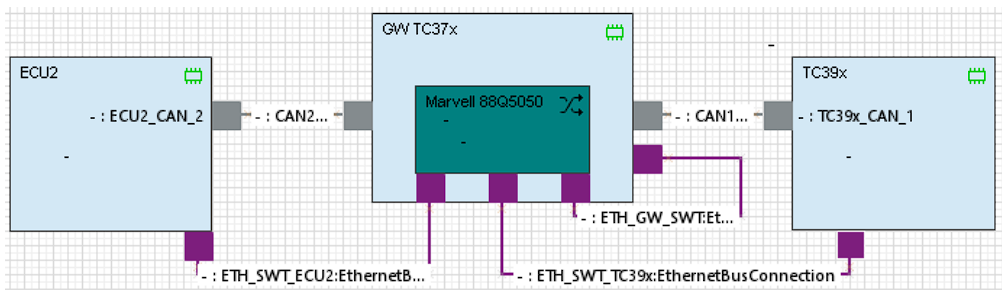
\includegraphics [width=5in]{img/GWDemoConnections.PNG}}
        \subfigure[Details des connections Ethernet du gateway]{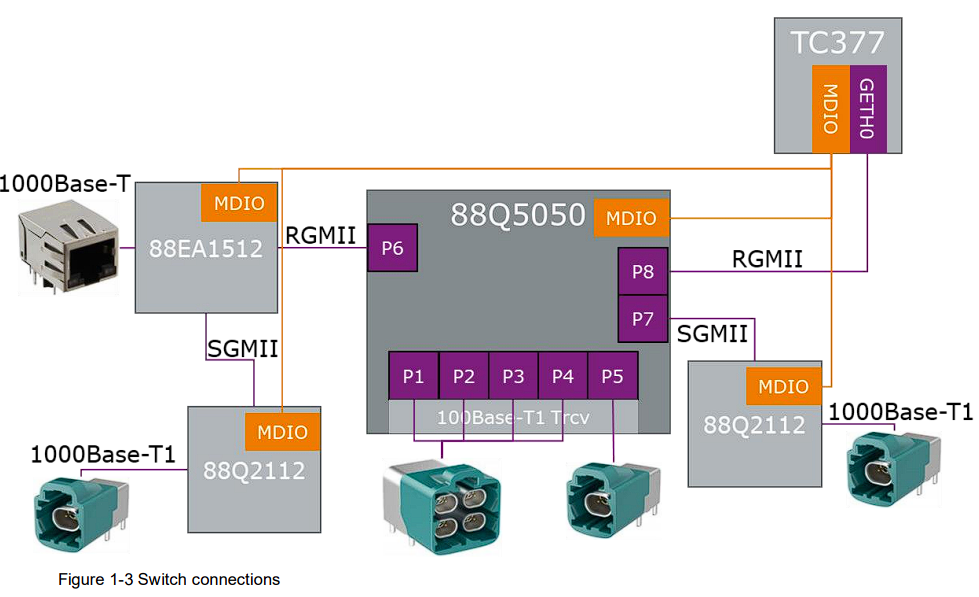
\includegraphics [width=5in]{img/eth_connections.png}}
    \caption{Appareils du demo technique}
    \label{fig:devices-diagram}
\end{figure}


\begin{figure}[!htb]
 \centering
 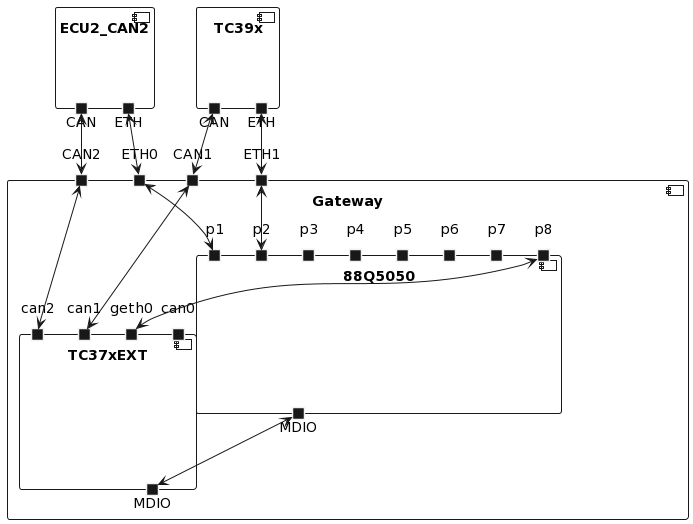
\includegraphics[width=\textwidth]{img/GWConnectionsDiagram.png}
 \caption{Gateway Connections Diagram}
 \label{fig:connections-diagram}
\end{figure}

\begin{figure}[!htb]
 \centering
 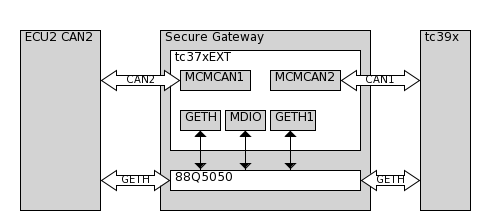
\includegraphics[width=\textwidth]{img/gateway_block_diagram.png}
 \caption{Gateway Block diagram}
 \label{fig:block diagram}
\end{figure}

\subsubsection{Switch Marvell 88Q5050}

Avant de demarrer les SWC le logiciel de la gateway verifie si toutes les composants et buses de donn\'ees sont presents. Un des composants present dans la carte est le Switch ethernet Marvell 88Q5050\cite{sw88Q5050}. C'est un switch securis\'e optimis\'e pour \^etre utilis\'e dans l'industrie automobile. Il est connect\'e aux ECUs externes via ports Ethernet et avec l'aurix a travers d'un port ethernet et un bus MDIO\cite{mdio-background}. Ce bus MDIO est utilis\'e pour accéder aux registres du switch a travers de l'aurix. De cette façon nous pouvons gérer le fonctionnement interne du switch avec l'aurix.

Ce modele a \'et\'e developp\'e en C++ et SystemC \`a l'aide du datasheet du fournisseur. Pour cette modèle j'ai suivi la procédure interne de modélisation des composants en ajoutant la quantit\'e  de buses, registres, ports et fonctionalit\'es de chaque élément. 

\subsubsection{Transceivers Marvell}

Ces transceivers montr\'es dans la fiugre \ref{fig:devices-diagram}\cite{88Q2112}\cite{88Q1010} connectent la couche PHY avec le switch. Avant le démarrage du logiciel le systeme de exploitation verifie son statut pour initialiser les ports.

Au moment de la rédaction de ce rapport, nous ne possédions pas les datasheet de ces transceivers. Dans la modèle du switch 88Q5050 est integr\'e les commandes necessarires pour "initialiser les transceivers".

%-------------------------- * Seccion de resultados * --------------------------------

\section{Resultats}

Los resultados son prometedores despues de 3 semanas.

Te habla el melet del futuro, le han salido tantas patas al gato que no has hecho ni la mitad de tu proyecto. Haz hecho mucho pero no has podido avanzar en el proyecto como tal

\subsection{Demarrage microsar}
Microsar al comienzo no queria arrancar porque el sistema simulado no soporta el BUS FlexRay tonces me toco "hackear" la tarjeta para que el sistema operativo viera que si lo soporta (incluso cuando no). Luego me toco hacer unas conexiones en el bus can y en el ASCLIN. 



%-------------------

%\begin{figure}[!htb]
%\centering
%\includegraphics[width=0.2\textwidth]{images/ubication-sipi.png}
%\caption{Location du village Sipí \cite{sipi:ubicacion}}
%\label{img:sipi:ubicacion}
%\end{figure}

%Para citar la bibliografia haces \cite{Photovoltaic}
%Para referenciar las imagenes haces lo sgte \ref{fig:schema}

\section{Conclusion}

\section{Anexes}
% ---- TC37x Delta ----
%\markdownInput{anexes/TC37xEXT_report.md}
%\label{anexe:tc37ex}

%debes hacer esto para meter archivos de otro lado
%\input{sub_files/Calcul_puissance}
%\label{anexe:calcul-puissance}
%-------------------

%Para meter un pdf haces lo sgte 
%\includepdf{images/Velocidad-Maxima-Energia_13}
%\label{pdf:vent_vitesse_max}
%-------------------

% \begin{figure}
%     \centering
%     \includegraphics[height=\textheight]{Anexes/RadiacionSolar13 (1).pdf}
%     \caption{Caption}
%     \label{fig:radiacion}
% \end{figure}


% Plantilla para colocar muchas imagenes con un multiplot
%\begin{figure}[!htb]
%\centering
%\subfigure[]{\includegraphics [width=2.5in]{lab_2_vision_15.png}}
%\subfigure[]{\includegraphics [width=2.5in]{lab_2_vision_16.png}}
%\subfigure[]{\includegraphics [width=2.5in]{lab_2_vision_17.png}}
%\caption{Paleta de colores}
%\end{figure}

% Plantilla para poner una imagen cualquiera
%\begin{figure}[!htb]
%\centering
%
%\caption{Histograma de la imagen}
%\end{figure}

\bibliography{Biblio}

\end{document}
